\documentclass[a4paper]{article}

\usepackage{cite}%多个文献引用
\usepackage{graphicx}
\usepackage{array}%调节表格行高
\usepackage{multirow,makecell}%多行表格
\usepackage{tabularx}%表格固定列宽
\usepackage{subfigure}
\usepackage{titlesec}%标题格式设置
\usepackage{amsmath}
\usepackage{amssymb}
\usepackage{tabularx}
\usepackage{makecell}
\usepackage{geometry}
\usepackage{float}
\usepackage{setspace}%行距包
\usepackage{siunitx}
\usepackage{mdwlist}
\usepackage{tabu}
\usepackage{enumerate}

\geometry{top=1.54cm,bottom=2.54cm,left=2.5cm,right=2.5cm}


\begin{document}
\begin{center}
\bf\Large
EE 105 Feedback Control Systems\par
Department of Electrical and Computer Engineering\par
Tufts University Fall 2018\par
Homework \#4\par   
\end{center}
\begin{table}[H]
\begin{center}
\begin{tabular*}{\textwidth}{@{\extracolsep{\fill}}lcr}
Name: {\it Shang Wang} &Student ID: {\it 1277417} &E-mail: {\it shang.wang@tufts.edu}\\
\hline
\end{tabular*}
\end{center}
\end{table}

\section{Problem 1}
Now use parameter $P$, $I$, $D$ instead of $B$, $K$, $M$. 
Write the transfer function of the system, use Black's formula, $C$ is the transfer function of controller while $P$ is the transfer function of the plant:
$$
H(s) = \frac{Y(s)}{R(s)} = \frac{CP}{1+CP} = \frac{Ds^2+Ps+I}{(m+D)s^2+(P+b)s+I}
$$
Since the input is a unit step function, if we use the final value theorem($D,P,I\neq 0$):
$$
y(\infty) = \lim_{s\rightarrow 0}s\cdot \frac1s H(s) = \frac{I}{I} = 1
$$
So if we want the system have zero steady-state error, the coefficient $I$ can not be zero, because if $I = 0$:
$$
y(\infty) = \lim_{s\rightarrow 0}s\cdot \frac1s H(s) = \frac{P}{P+b}<1
$$
Using the initial value theorem:
$$
y(0) = \lim_{s\rightarrow \infty}s\cdot \frac1s H(s) = \frac{D}{m+D}
$$
So if we do not want the system have abrupt jump at $t = 0$, $D$ must be zero. Thus, the transfer function of the system becomes:
$$
H(s) = \frac{Ps+I}{ms^2+(P+b)s+I}
$$
Poles at:
$$
s_p = -\frac{P+b}{2m}\pm \frac{1}{2m}\sqrt{(P+b)^2-Im}
$$
Zeros at:
$$
s_z = -\frac IP
$$
Rewrite the system transfer function:
$$
H(s) = \frac{P}{m}\frac{s+\frac IP}{s^2+2\zeta \omega_n + \omega_n^2}
$$
Where:
$$
\omega_n = \sqrt{\frac Im},\ \ \zeta = \frac{P+b}{2\sqrt{mI}}
$$
Ignore the zeros, focus on the poles. We need an underdamped second order system with the rising time no more than 20s and overshoot less than 10\%. Damping ratio has to be between 0 and 1. We can solve the overshoot equation:
$$
e^{-\pi\zeta/\sqrt{1-\zeta^2}} = 10\%
$$
We have a solution $\zeta = 0.59155$. Then solve the rising time equation:
$$
\frac{\pi-\arccos(\zeta)}{\omega_n\sqrt{1-\zeta^2}} = 20
$$
We have the value of $\omega_n = 0.1366$. Therefore, 
$$
I = 18.66,\ \ P = 111.6
$$
As the plots show, the zeros will seriously affect the performance of the system because the zeros is near these poles. Therefor, we have overshoot more than 10\% due to the zeros. One way to fix this is to increase the damping ratio $\zeta$. The plot with the notation "no zeros" is the plot with the transfer function of $\omega_n^2/(s^2+2\zeta \omega_n + \omega_n^2)$, which can easily see the difference with the practical transfer function $H(s)$. 
\begin{figure}[H]
\centering
\begin{minipage}[t]{0.48\textwidth}
\centering
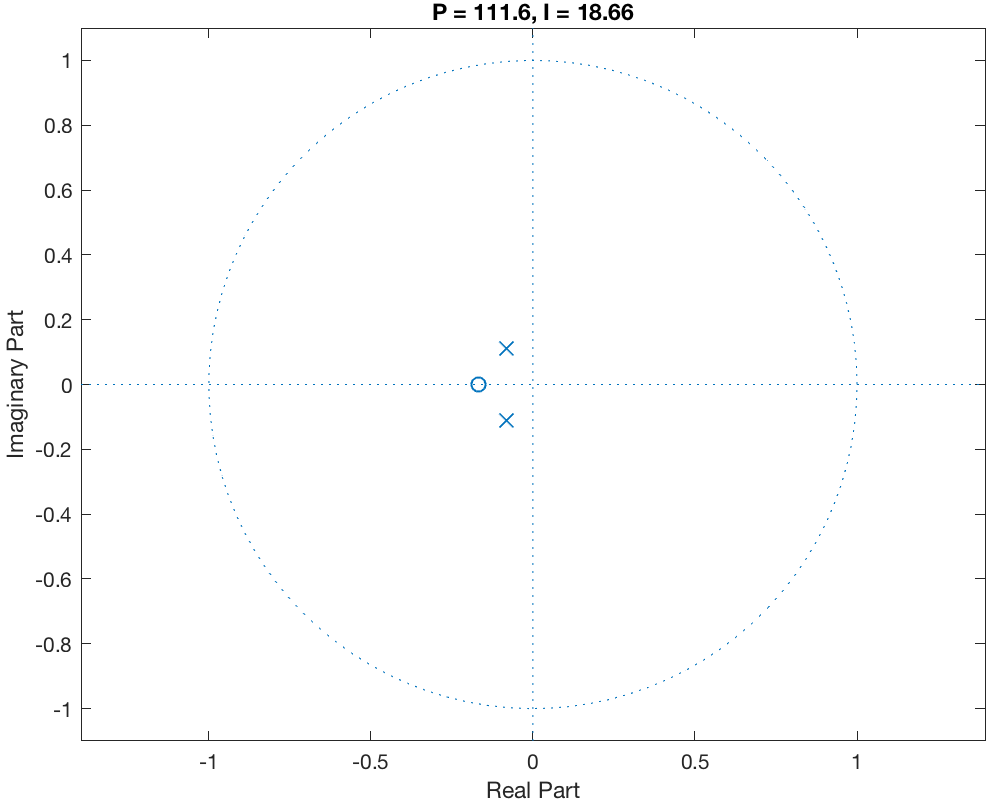
\includegraphics[width=\textwidth]{pic/zp1.png}
\caption{zeros and poles}
\end{minipage}
\begin{minipage}[t]{0.48\textwidth}
\centering
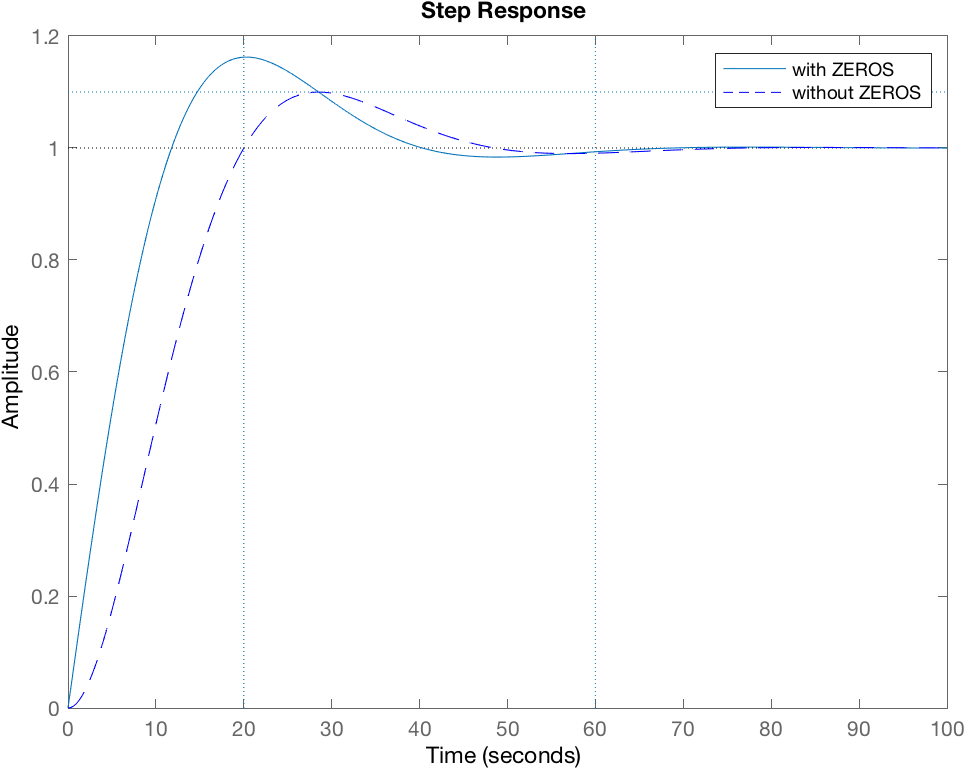
\includegraphics[width=\textwidth]{pic/zo1.png}
\caption{Step response for $P = 111.6$, $I = 18.66$}
\end{minipage}
\end{figure}
\noindent If we adjust the parameter a bit, like increasing the damping ratio a little by increasing the coefficient $P$. 
$$
I = 18.66,\ \ P = 160
$$
Plots are like these, which have basically satisfied the requiments.
\begin{figure}[H]
\centering
\begin{minipage}[t]{0.48\textwidth}
\centering
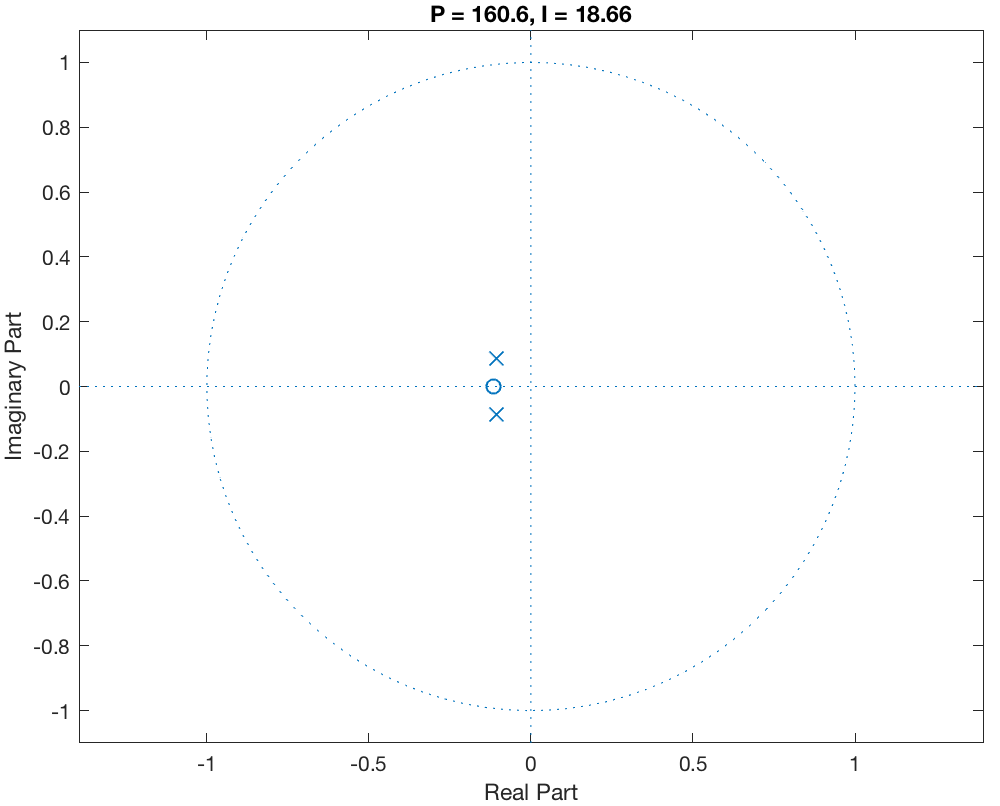
\includegraphics[width=\textwidth]{pic/zp2.png}
\caption{zeros and poles}
\end{minipage}
\begin{minipage}[t]{0.48\textwidth}
\centering
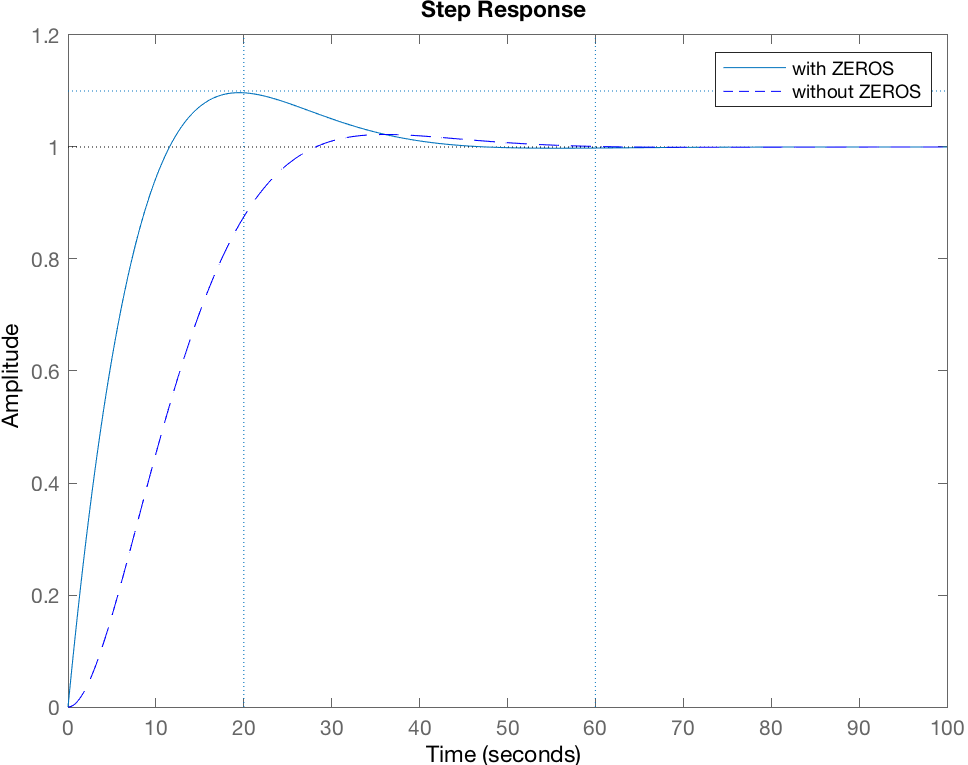
\includegraphics[width=\textwidth]{pic/zo2.png}
\caption{Step response for $P = 160.6$, $I = 18.66$}
\end{minipage}
\end{figure}










\end{document}